\documentclass[11pt,a4paper]{article}

\usepackage[T1]{fontenc}
\usepackage[utf8]{inputenc}
\usepackage{lmodern}
\usepackage{microtype}
\usepackage[margin=2.3cm]{geometry}
\usepackage{graphicx}
\usepackage{booktabs}
\usepackage{tabularx}
\usepackage{array}
\usepackage{xcolor}
\usepackage{listings}
\usepackage{tikz}
\usetikzlibrary{arrows.meta,positioning,fit}
\usepackage{pgfplots}
\pgfplotsset{compat=1.18}
\usepackage{enumitem}
\usepackage{caption}
\usepackage[hidelinks]{hyperref}

\definecolor{accent}{HTML}{1C5CAB}
\definecolor{muted}{HTML}{6B6B66}
\definecolor{codebg}{HTML}{F4F3EF}
\captionsetup{font=small,labelfont=bf}
\setlist{itemsep=2pt,topsep=4pt}
\lstset{basicstyle=\ttfamily\small,backgroundcolor=\color{codebg},frame=none,columns=fullflexible,
        breaklines=true,xleftmargin=6pt,framexleftmargin=6pt,aboveskip=6pt,belowskip=6pt}
\newcommand{\code}[1]{\texttt{#1}}
\sloppy
\newcommand{\screenshot}[3]{%
  \begin{figure}[htbp]\centering
  \fbox{\includegraphics[width=0.94\linewidth,height=0.62\textheight,keepaspectratio]{figures/#1}}
  \caption{#2}\label{#3}\end{figure}}

% Written by report/measure.py. Do not edit.
\newcommand{\mPapers}{12}
\newcommand{\mSections}{120}
\newcommand{\mWords}{78,625}
\newcommand{\mPassages}{1591}
\newcommand{\mQuotes}{37}
\newcommand{\mQuotesVerified}{33}
\newcommand{\mQuotesPct}{89}
\newcommand{\mTimed}{11}
\newcommand{\mTimeMin}{2.7}
\newcommand{\mTimeMax}{35.9}
\newcommand{\mTimeMedian}{28.7}
\newcommand{\mTimeMean}{25.2}
\newcommand{\mWaits}{12}
\newcommand{\mWaitSeconds}{250}
\newcommand{\mCited}{11}
\newcommand{\mAuthors}{65}
\newcommand{\mPairs}{212}
\newcommand{\mDensity}{0.102}
\newcommand{\mGroups}{11}
\newcommand{\mLargestGroup}{17}
\newcommand{\mRecurring}{3}
\newcommand{\mPaperRows}{%
1706.03762 & Attention Is All You Need & 2017 & 8 & 4,113 & 71 & 40 & 202,845 & 3/3 & 2.7 \\
2004.04906 & Dense Passage Retrieval for Open-Domain\,\ldots & 2020 & 13 & 6,293 & 115 & 48 & 7,897 & 3/4 & 8.9 \\
2005.11401 & Retrieval-Augmented Generation for\,\ldots & 2020 & 17 & 6,409 & 114 & 68 & 21,066 & 3/4 & 30.6 \\
2007.01282 & Leveraging Passage Retrieval with\,\ldots & 2020 & 5 & 2,331 & 39 & 34 & 2,257 & 3/3 & 24.8 \\
2212.10496 & Precise Zero-Shot Dense Retrieval without\,\ldots & 2022 & 7 & 3,359 & 59 & 39 & 1,080 & 4/4 & 35.9 \\
2309.15217 & Ragas: Automated Evaluation of Retrieval\,\ldots & 2023 & 7 & 3,114 & 52 & 28 & 1,373 & 3/3 & -- \\
2310.11511 & Self-RAG: Learning to Retrieve, Generate,\,\ldots & 2023 & 11 & 12,443 & 400 & 58 & 3,121 & 3/3 & 31.0 \\
2312.10997 & Retrieval-Augmented Generation for Large\,\ldots & 2023 & 8 & 9,454 & 179 & 182 & 4,508 & 3/3 & 28.9 \\
2401.15884 & Corrective Retrieval Augmented Generation & 2024 & 8 & 6,124 & 111 & 41 & 360 & 2/2 & 28.7 \\
2404.10981 & A Survey on Retrieval-Augmented Text\,\ldots & 2024 & 10 & 11,542 & 218 & 166 & 217 & 1/3 & 30.0 \\
2405.07437 & Evaluation of Retrieval-Augmented\,\ldots & 2024 & 6 & 5,880 & 108 & 77 & 358 & 2/2 & 28.1 \\
2611.17161 & Cited but Unused: Parametric Provenance in\,\ldots & 2026 & 20 & 7,563 & 125 & 53 & -- & 3/3 & 27.6 \\
}


\title{\textbf{An AI Research Assistant for Reading Papers}\\[4pt]
\large Rebuilding \code{AI-Research-Assistant-New} around real arXiv papers, a real language model,\\
and output a professor can check}
\author{Kunal Jangid\\
\normalsize Roll no.\ B23MT1026\\[2pt]
\normalsize CSD4020: AI Specialisation Project}
\date{November 2026}

\begin{document}
\maketitle

\begin{abstract}
\noindent The original repository presented itself as an AI research assistant but analysed a folder of
hand-written JSON records, used placeholder language models and embeddings whenever no OpenAI key was set,
and reported metrics that did not measure what their names said. This report describes the replacement: a
Streamlit application that searches arXiv through its API, reads each paper's full text from arXiv's HTML
rendering with BeautifulSoup, indexes it with a local embedding model, and uses an LLM on Groq's free tier to
write digests, answer questions with cited passages and compare papers. It is designed around a professor's
reading workflow: deciding what to read, understanding it quickly, checking what the model claims, and
reusing the result in teaching and writing. On a library of \mPapers{} papers (\mWords{} words of extracted
text), \mQuotesVerified{} of the \mQuotes{} supporting quotes in the generated digests (\mQuotesPct\%) were
found word for word in the source paper. Questions are answered by a hybrid pipeline --- BM25 and dense
search in FAISS, fused by reciprocal rank and re-ranked by a cross-encoder --- behind input, context and
output guardrails. An ablation study over six chunking strategies, nine embedding models, four re-rankers
and five vector stores chose its settings; on 77 questions with known evidence it raises retrieval MRR
from 0.52 to 0.66 and brings the evidence to the model for 87\% of questions instead of 71\%. Ragas scores
the answers before and after.
\end{abstract}

\tableofcontents
\bigskip

%=====================================================================
\section{Starting point}

The repository contained four entry scripts (\code{fixed\_assistant.py}, \code{interactive\_assistant.py},
\code{docker\_assistant.py}, \code{docker\_interactive.py}), a plotting module, a Docker set-up and a
\code{research-db/} folder of paper records. Running it and reading the code showed five problems.

\begin{description}[leftmargin=0pt]
\item[The AI was a placeholder.] Without a key beginning \code{sk-}, the code fell back to LangChain's
  \code{FakeListLLM}, which returns canned strings in rotation, and \code{FakeEmbeddings}, which returns
  random vectors. The ``insights'' a user saw were therefore not derived from the papers.
\item[The papers were not real.] Papers were loaded only from JSON files in \code{research-db/}, written by
  hand with fields such as \code{keywords} and \code{citations}. There was no search and no way to add a
  real paper.
\item[The metrics did not measure their names.] ``Collaboration index'' was papers divided by authors,
  capped at 1; ``trend velocity'' was the number of papers divided by ten; ``diversity'' was the ratio of
  distinct keywords to keywords; ``impact'' averaged the hand-entered citation field.
\item[Docker could not run.] The Dockerfile was built on a Terminal-Bench base image, and the compose file
  ran a \code{solution.sh} that is not in the repository, with log paths taken from benchmark environment
  variables.
\item[A credential was committed.] \code{docker-compose.yaml} contained a literal \code{LANGCHAIN\_API\_KEY}
  value. It should be treated as leaked and revoked by its owner; deleting the file does not remove it from
  the Git history.
\end{description}

All of these files were removed. What replaced them is described below.

%=====================================================================
\section{What a professor needs from such a tool}

New papers appear faster than anyone can read them. A professor typically has to:
\begin{enumerate}
\item \textbf{triage}: notice the few new papers that matter to their research, out of hundreds a week;
\item \textbf{understand} a chosen paper quickly, sometimes from outside their own speciality;
\item \textbf{check} anything a summary claims before repeating it to students or in a review;
\item \textbf{reuse} what they read: in a lecture, a reading group, a referee report or a related-work section.
\end{enumerate}
A language model helps with all four, but only if its output can be traced to the paper. That principle
shaped the design: every generated statement is either tied to quoted text that the application checks, or
to numbered passages that are shown next to the answer. Figures on the Insights page are computed, never
generated.

\begin{table}[htbp]\centering\small
\begin{tabularx}{\linewidth}{@{}l>{\raggedright\arraybackslash}X>{\raggedright\arraybackslash}X@{}}
\toprule
Need & Feature & Where \\
\midrule
Triage & Search ranked by similarity to a written statement of research interests; a watchlist of followed
  searches; a briefing that rates each new paper high/medium/low for this reader with a reason &
  Discover \\
Understand & Digest at two depths, written for a specialist, a neighbouring field or a graduate student;
  background needed; questions answered from the paper & Reader \\
Check & Each key result carries a quote that is matched against the paper text; answers cite numbered
  passages shown beside them; full extracted text is browsable & Reader \\
Reuse & Discussion questions for a reading group; side-by-side comparison; related-work paragraph with
  numbered references; BibTeX and Markdown export; personal notes, tags and reading status &
  Reader, Synthesize, Library \\
Overview & Timeline, categories, characteristic terms, topic map, co-author network, citation counts &
  Insights \\
\bottomrule
\end{tabularx}
\caption{The reading workflow and the feature that serves each step.}
\end{table}

%=====================================================================
\section{Architecture}

\begin{figure}[htbp]\centering
\resizebox{\linewidth}{!}{%
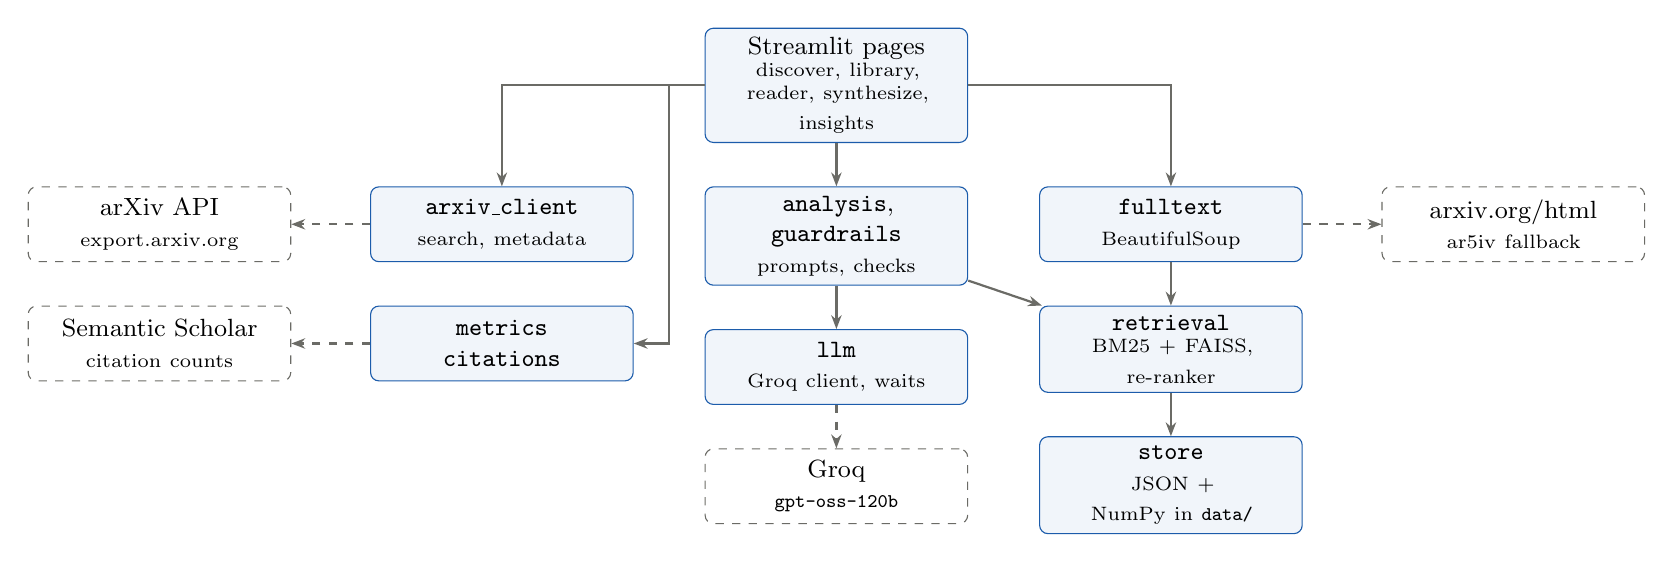
\begin{tikzpicture}[
  box/.style={draw=accent,rounded corners=3pt,fill=accent!6,align=center,font=\small,minimum height=0.95cm,
              text width=3.1cm},
  ext/.style={draw=muted,dashed,rounded corners=3pt,align=center,font=\small,minimum height=0.95cm,
              text width=3.1cm},
  arr/.style={-{Stealth[length=5pt]},thick,muted}, node distance=0.55cm and 0.9cm]
\node[box] (ui) {Streamlit pages\\\scriptsize discover, library,\\reader, synthesize,\\insights};
\node[box,below left=of ui] (arx) {\code{arxiv\_client}\\\scriptsize search, metadata};
\node[box,below=of ui] (an) {\code{analysis}, \code{guardrails}\\\scriptsize prompts, checks};
\node[box,below right=of ui] (ft) {\code{fulltext}\\\scriptsize BeautifulSoup};
\node[box,below=of arx] (met) {\code{metrics}\\\code{citations}};
\node[box,below=of an] (llm) {\code{llm}\\\scriptsize Groq client, waits};
\node[box,below=of ft] (ret) {\code{retrieval}\\\scriptsize BM25 + FAISS,\\re-ranker};
\node[box,below=of ret] (st) {\code{store}\\\scriptsize JSON + NumPy in \code{data/}};
\node[ext,left=1.0cm of arx] (xa) {arXiv API\\\scriptsize export.arxiv.org};
\node[ext,left=1.0cm of met] (xs) {Semantic Scholar\\\scriptsize citation counts};
\node[ext,right=1.0cm of ft] (xh) {arxiv.org/html\\\scriptsize ar5iv fallback};
\node[ext,below=of llm] (xg) {Groq\\\scriptsize \code{gpt-oss-120b}};
\draw[arr] (ui.west) -| (arx); \draw[arr] (ui) -- (an); \draw[arr] (ui.east) -| (ft);
\draw[arr] (ui.west) -- ++(-4.5mm,0) |- (met.east); \draw[arr] (an) -- (llm); \draw[arr] (an) -- (ret); \draw[arr] (ft) -- (ret);
\draw[arr] (ret) -- (st);
\draw[arr,dashed] (arx) -- (xa); \draw[arr,dashed] (met) -- (xs);
\draw[arr,dashed] (ft) -- (xh); \draw[arr,dashed] (llm) -- (xg);
\end{tikzpicture}}
\caption{Modules of the \code{research\_assistant} package and the services they call. Dashed boxes are
external. Embeddings are computed locally; only the LLM call leaves the machine with paper text.}
\label{fig:arch}
\end{figure}

The code is a small Python package used by five Streamlit pages (Figure~\ref{fig:arch}). Each module has one
job, and nothing in the package imports Streamlit except \code{ui.py}, so every module is tested without a
running app. A saved paper is one JSON file (metadata, extracted sections, digests, notes, status) and one
compressed NumPy file (its passages, their vectors and the settings they were built with). The library-wide
FAISS and BM25 indexes are assembled from those files in memory and rebuilt when one changes. There is no
database server: a reading library holds hundreds of papers, not millions, and
Section~\ref{sec:stores} measures what a vector database would and would not add.

%=====================================================================
\section{Getting real papers}

\subsection{Search and metadata: the arXiv API}
\code{arxiv\_client.py} builds queries for the Atom API at \code{export.arxiv.org/api/query}. Quoted phrases
are kept as phrases, other words are joined with \code{AND}, a search can be limited to title, abstract,
author or all fields, and to one of sixteen arXiv categories, and results can be sorted by relevance,
submission date or last update. The feed is parsed with the standard library's XML parser into a
\code{Paper} record: identifier and version, title, authors, abstract, dates, primary and secondary
categories, comment, journal reference and DOI. arXiv reports query errors as a feed entry rather than an
HTTP status; those are raised as errors instead of being shown as a paper. Calls are spaced at least three
seconds apart, as arXiv's terms of use ask, and every request carries a descriptive User-Agent.

\subsection{Full text: BeautifulSoup on arXiv's HTML}
Abstracts are not enough to digest a paper. arXiv renders most recent submissions to HTML with LaTeXML at
\code{arxiv.org/html/<id>}, and the ar5iv project covers many older ones. \code{fulltext.py} fetches the first
of the two that exists and walks the document with BeautifulSoup, relying on LaTeXML's \code{ltx\_*} classes:
\begin{itemize}
\item sections (\code{ltx\_section}, appendices) become \code{Section(title, text)}; subsection headings are
  kept inline as \code{\#\#} lines so retrieved passages still say where they came from;
\item mathematics is replaced by its LaTeX source from the \code{alttext} attribute, written as
  \code{\$\ldots\$}, so formulas survive as text the model can read;
\item footnotes, author blocks and navigation are removed; data tables are removed (their cells are
  unreadable once flattened) but their captions are kept in brackets, as are figure captions; equation
  tables are kept;
\item the bibliography is counted, not included.
\end{itemize}
A page with fewer than 1,500 characters of body text is rejected, so a stub or an error page is never taken
for a paper. When neither source has the paper it is saved with its abstract only, marked as such in the
interface, and offered a retry.

%=====================================================================
\section{Retrieval}\label{sec:retrieval}

\begin{figure}[htbp]\centering
\resizebox{\linewidth}{!}{%
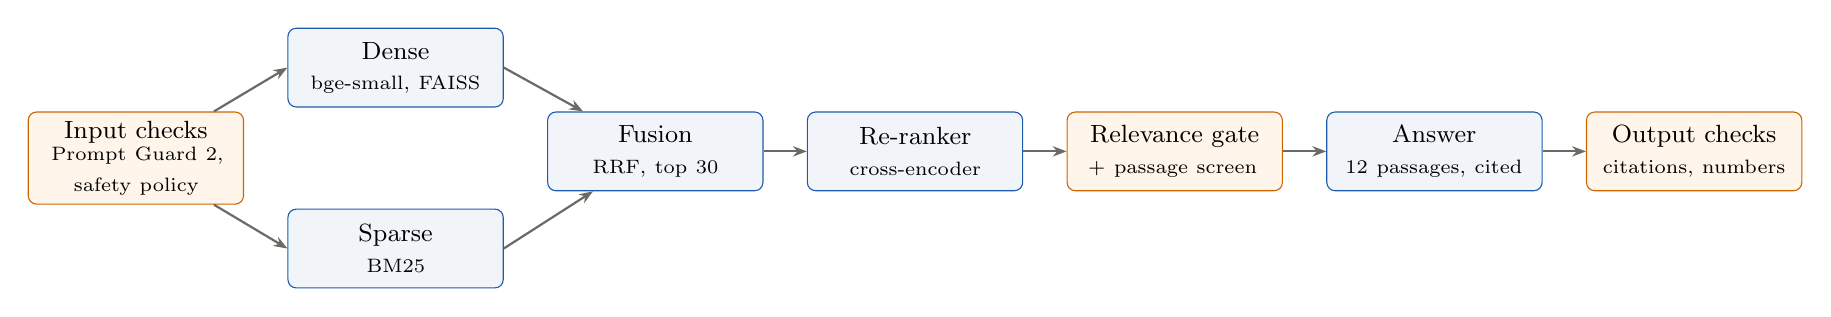
\begin{tikzpicture}[
  box/.style={draw=accent,rounded corners=3pt,fill=accent!6,align=center,font=\small,minimum height=1.0cm,text width=2.5cm},
  gate/.style={draw=orange!80!black,rounded corners=3pt,fill=orange!8,align=center,font=\small,minimum height=1.0cm,text width=2.5cm},
  arr/.style={-{Stealth[length=5pt]},thick,muted}, node distance=0.5cm and 0.55cm]
\node[gate] (in) {Input checks\\\scriptsize Prompt Guard 2,\\safety policy};
\node[box,above right=0.05cm and 0.55cm of in] (dense) {Dense\\\scriptsize bge-small, FAISS};
\node[box,below right=0.05cm and 0.55cm of in] (bm) {Sparse\\\scriptsize BM25};
\node[box,below right=0.05cm and 0.55cm of dense] (rrf) {Fusion\\\scriptsize RRF, top 30};
\node[box,right=of rrf] (ce) {Re-ranker\\\scriptsize cross-encoder};
\node[gate,right=of ce] (g) {Relevance gate\\\scriptsize + passage screen};
\node[box,right=of g] (llm) {Answer\\\scriptsize 12 passages, cited};
\node[gate,right=of llm] (out) {Output checks\\\scriptsize citations, numbers};
\draw[arr] (in) -- (dense.west); \draw[arr] (in) -- (bm.west);
\draw[arr] (dense.east) -- (rrf); \draw[arr] (bm.east) -- (rrf);
\draw[arr] (rrf) -- (ce); \draw[arr] (ce) -- (g); \draw[arr] (g) -- (llm); \draw[arr] (llm) -- (out);
\end{tikzpicture}}
\caption{The question-answering pipeline. Blue stages retrieve and answer; orange stages are the guardrails
of Section~\ref{sec:guardrails}. Every setting was chosen by the ablation study in Section~\ref{sec:ablation}.}
\label{fig:pipeline}
\end{figure}

The first version embedded each question and returned the passages with the highest cosine similarity.
Dense retrieval is good at paraphrase but weak on the exact terms that dominate research questions ---
dataset names, metric names, model names, numbers --- so the pipeline is now hybrid (Figure~\ref{fig:pipeline}):
\begin{enumerate}
\item \textbf{Chunking.} Each paper is split into passages of at most 512 characters on sentence boundaries
  with 64 characters of overlap, each prefixed by its section title; the abstract is the first passage.
  The \mPapers{} papers of Section~\ref{sec:results} give \mPassages{} passages.
\item \textbf{Dense search.} Passages are embedded with \code{BAAI/bge-small-en-v1.5} through
  \code{fastembed}, an ONNX runtime that needs no GPU and no PyTorch, with the model's instruction prefix on
  the query side only. Vectors are L2-normalised and held in a FAISS \code{IndexFlatIP}, so the inner product
  is the cosine similarity and the search is exact; a restriction to one paper is an \code{IDSelectorBatch}.
\item \textbf{Sparse search.} Okapi BM25 ($k_1=1.5$, $b=0.75$) over the same passages, implemented on
  scikit-learn's \code{CountVectorizer} with the term weights precomputed in a sparse matrix, so scoring a
  query is one column sum (about 0.2~ms).
\item \textbf{Fusion.} Reciprocal Rank Fusion, $\sum_r 1/(60+\mathrm{rank}_r)$, combines the two rankings
  without having to calibrate their scores against each other; the best 30 are kept.
\item \textbf{Re-ranking.} A cross-encoder (\code{ms-marco-MiniLM-L-6-v2}) reads each question--passage
  pair together and re-orders the 30 candidates. The best 12 (about 5,300 characters) go to the model, or
  16 when the question is about the whole library.
\end{enumerate}
Changing the chunking or the embedding model in \code{config.py} re-indexes the saved papers on the next
search: each index file records the settings it was built with.

The same model ranks search results against the reader's interests: the professor writes a few sentences
about their research once, and each abstract is scored by its cosine similarity to that statement. The
score orders results; the interface says explicitly that it is not a percentage.

%=====================================================================
\section{Using a language model on a free tier}

\subsection{Model and limits}
The LLM is \code{openai/gpt-oss-120b} on Groq, called through its OpenAI-compatible endpoint with the
\code{openai} SDK and low reasoning effort. The key is read from \code{GROQ\_API\_KEY} or
\code{GROQ\_CLOUD\_API\_KEY} in \code{.env}, or from Streamlit secrets when deployed. Groq's free tier allows
8,000 tokens per minute, counting prompt and completion together, which shapes everything else:
\begin{itemize}
\item a single request carries at most about 15,000 characters of paper text and asks for at most 1,800
  output tokens;
\item when the limit is hit, the client reads the wait Groq asks for (the \code{retry-after} header, or the
  ``try again in \ldots'' message), waits, tells the user it is waiting, and tries again; a request that is
  too large for the tier is reported as such rather than retried;
\item streaming is used for answers, so text appears as it is written.
\end{itemize}

\subsection{Two depths of digest}
A whole paper does not fit in one request, so the reader chooses:
\begin{description}
\item[Focused] (one call): the abstract, the introduction, up to two closing sections (conclusion,
  discussion, limitations) and the passages retrieved for three questions --- the method, the main results
  with numbers, and limitations --- until the character budget is used.
\item[Full paper] (one call per block of about 12,000 characters, then one more): the model first takes
  reading notes on each block, keeping every quantitative result and copying key sentences verbatim; the
  digest is then written from all the notes. A 12,000-word paper needs five or six calls and, on the free
  tier, a few minutes.
\end{description}
Each digest records which text it was written from, and the interface shows it.

\subsection{Structured output that can be checked}
Digests, comparisons and briefings are requested as JSON objects with named fields. Model output is not
always well formed, so:
\begin{itemize}
\item the parser accepts code fences and surrounding prose and extracts the object;
\item an answer wrapped in an extra object is unwrapped; an answer missing a required field is requested
  once more and otherwise reported as an error --- an empty box is never shown as if the model had found
  nothing (this fixed an intermittent empty ``Where they agree'' panel on the Synthesize page);
\item digest fields are coerced to their types (a string where a list was asked for becomes a one-item list,
  a null becomes empty), so exports cannot fail on an unexpected shape.
\end{itemize}

\subsection{Quote verification}
Each key result in a digest has two parts: a one-sentence claim and a quote of at most 30 words that the
model is told to copy exactly. The application then searches the paper's text for the quote after
lower-casing, collapsing whitespace and punctuation, and dropping full stops other than decimal points. A
quote with an ellipsis passes when every fragment of 15 or more characters is found. The result is shown on
each card as ``Quote found in the paper'' or ``Not found word for word'' (Figure~\ref{fig:digest}).

This check has a precise and limited meaning. A match shows that the quoted words are in the paper, not that
the claim follows from them; the reader still has to compare the two, which is why they are displayed
together. A miss usually means paraphrase rather than invention (Section~\ref{sec:results}).

\subsection{Answers with sources}
In the Ask view, the question passes the input checks, the pipeline of Section~\ref{sec:retrieval} finds
twelve passages of the paper (or sixteen across the whole library), and they are numbered and sent inside
\code{<passage n="i">} tags with the instruction to cite them as [1], [2], to treat their content as data
rather than instructions, and to say so when they do not contain the answer. The passages are shown beneath the answer with their section names, so every
citation can be followed (Figure~\ref{fig:ask}). The last four turns of the conversation are included so
follow-up questions work.

%=====================================================================
\section{Guardrails}\label{sec:guardrails}

A reading assistant takes text from two untrusted places: the question, and the papers themselves, which
may quote prompt-injection attacks or contain hidden instructions. \code{guardrails.py} checks at three
points, and the interface shows every check as a step under the answer (Figure~\ref{fig:ask}).
\begin{description}
\item[Input.] The question is stripped of control and invisible formatting characters (a way to hide
  instructions) and limited to 1,000 characters. Two Groq-hosted classifiers then run in parallel:
  Llama Prompt Guard~2 (86M) returns the probability of a prompt attack, blocking at 0.5, with a regular
  expression as the fallback when it cannot be reached; and \code{gpt-oss-safeguard-20b} classifies the
  question against a short written policy (weapons capable of mass harm, malware, sexual content involving
  minors, self-harm, hate), which explicitly allows academic discussion of those topics. The safety check
  fails open, since an outage should not stop a professor reading a paper.
\item[Context.] If the best re-ranker score is below $-5$, no passage is relevant enough and the
  application says the papers do not contain the answer \emph{without calling the model}; the threshold was
  calibrated on answerable and unanswerable questions (Section~\ref{sec:guardeval}). Retrieved passages with
  instruction-like text are flagged but kept --- papers about prompt injection quote attacks --- and the
  prompt frames all paper text as data.
\item[Output.] Citations must refer to passages that exist; every factual sentence should carry one;
  every number of two or more digits in the answer must occur in the passages; and an answer that echoes
  the system prompt or an API key is withheld. Only the last blocks; the others are shown as warnings,
  because a professor is better served by a visible flag than by a missing answer.
\end{description}

%=====================================================================
\section{The interface}

The application uses Streamlit 1.67 with top navigation between five pages, a light and a dark theme
defined in \code{.streamlit/config.toml} (Inter for the interface, Source Serif~4 for headings, JetBrains
Mono for code), and Material icons. Streamlit's bundled \emph{developing-with-streamlit} skill was followed
for layout and widget choice: segmented controls for exclusive views, pills for status filters, dialogs
for destructive actions, compact status indicators for long operations, \code{st.write\_stream} for
answers, and the selected paper bound to the URL so a reader view can be bookmarked or shared.

\screenshot{discover.png}{Discover. Results from the arXiv API, ordered by cosine similarity to the
professor's interests statement. Papers already saved are marked and open in the reader.}{fig:discover}

\screenshot{library.png}{Library. Saved papers with reading status, tags, whether full text was extracted,
and citation counts; several rows can be selected to change status, export BibTeX or remove.}{fig:library}

\screenshot{reader_digest.png}{Reader, Digest view. Depth and audience are chosen above the digest. Each key
result shows the model's claim, the quote it gave, and whether that quote was found in the paper.}{fig:digest}

\screenshot{reader_ask.png}{Reader, Ask view. The status line expands into the checks made before the
model was called (question screened; twelve passages found by hybrid search and re-ranking, the best scoring
0.52, none with planted instructions). The answer cites passage [2]; the guardrail panel below it flags that
its first sentence carries no citation. The passages are listed underneath.}{fig:ask}

\screenshot{synthesize.png}{Synthesize, comparing five saved papers: a side-by-side table, agreements,
differences and open questions, and a related-work paragraph with its numbered references. Both the
paragraph and the BibTeX can be downloaded.}{fig:synth}

%=====================================================================
\section{Visualisations and their accuracy}

The Insights page (Figures~\ref{fig:ins1}--\ref{fig:dark}) answers ``what is in my library?''. Each chart was
chosen for what it has to show, and each states in a caption what it measures and what it does not.

\begin{description}[leftmargin=0pt]
\item[Papers over time.] A bar chart of counts by month or, beyond three years, by year of first
  submission. Empty periods are filled with zeros so gaps are visible rather than closed up.
\item[Categories.] Horizontal bars of primary arXiv category, sorted. Each paper is counted once, so the
  bars sum to the number of papers.
\item[Characteristic terms.] Terms and two-word phrases ranked by mean TF-IDF weight over titles and
  abstracts, with English and academic stop words (``paper'', ``propose'', ``state-of-the-art'', \ldots)
  removed, terms in more than 85\% of papers dropped, and a term hidden when a higher-ranked phrase already
  contains it. Bar length is \emph{document frequency} --- the number of papers containing the term --- which
  can be read directly, rather than a TF-IDF weight, which cannot.
\item[Topic map.] Abstract embeddings are clustered with $k$-means, $k$ from 2 to 4 chosen by silhouette
  score, and drawn in two dimensions with PCA. Groups are labelled with their most characteristic terms and
  distinguished by shape as well as colour. The caption gives the silhouette score and the share of variance
  the projection keeps (46\% for the library shown) and says that the axes have no units. With fewer than
  six papers the map is not drawn.
\item[Co-author network.] An interactive force-directed graph: a line joins authors of the same saved paper,
  thicker for more joint papers, larger dots for authors of more papers. Above it are counts that can be
  checked by hand: \mAuthors{} authors, \mPairs{} co-author pairs, density \mDensity, \mGroups{} separate groups
  (the largest has \mLargestGroup{} authors), and \mRecurring{} authors who appear in more than one paper.
\item[Citations.] Counts from Semantic Scholar, refreshed on demand. Citation counts are heavily skewed ---
  from 217 to 202,845 here --- so when the largest is more than 50 times the smallest the chart switches to
  dots on a logarithmic axis with ticks at powers of ten and exact values as labels; otherwise it uses bars.
  The caption notes that older papers have had longer to be cited and that this is not a quality ranking.
\end{description}

\noindent\textbf{Colour.} Categorical colours follow a fixed order and stay attached to their category; the
palette was checked with a colour-vision-deficiency validator in both light and dark mode and passed
(lightness band, chroma, adjacent-pair separation under simulated deuteranopia, protanopia and tritanopia,
and contrast against the surface). The dark theme uses its own colours checked against the dark surface,
not an inversion. Text in charts uses the theme's ink, never the series colour; a check of the dark theme
found the citation labels drawn in Vega's default black, and they now take the theme's text colour.

\screenshot{insights_top.png}{Insights, upper half: counts by year and category, characteristic terms by
document frequency, and the topic map with its silhouette score and retained variance stated.}{fig:ins1}

\screenshot{insights_bottom.png}{Insights, lower half: the co-author network with its summary counts, and
citation counts on a logarithmic axis.}{fig:ins2}

\screenshot{insights_dark_top.png}{The same charts in the dark theme, with colours chosen and checked for
the dark surface.}{fig:dark}

%=====================================================================
\section{Measurements}\label{sec:results}

\code{report/measure.py} produced the numbers in this section from the library used for the screenshots:
\mPapers{} papers on retrieval-augmented generation and its foundations, from 2017 to 2026, each saved
through the application. It writes \code{measurements.json} and the \code{measurements.tex} file that this
report reads, so the figures here are the script's output, not copied by hand.

\begin{table}[htbp]\centering\scriptsize
\setlength{\tabcolsep}{3.5pt}
\resizebox{\linewidth}{!}{%
\begin{tabular}{@{}llrrrrrrrr@{}}
\toprule
arXiv & Title & Year & Sections & Words & Passages & Refs & Citations & Quotes found & Digest (s) \\
\midrule
\mPaperRows
\midrule
\multicolumn{3}{@{}l}{Total} & \mSections & \mWords & \mPassages & & & \mQuotesVerified/\mQuotes & \\
\bottomrule
\end{tabular}}
\caption{Per-paper results. \emph{Words} and \emph{Sections} are of the text extracted from arXiv HTML;
\emph{Refs} counts bibliography entries; \emph{Citations} are from Semantic Scholar (-- = not indexed yet);
\emph{Quotes found} is how many supporting quotes in the focused, specialist digest were found in the paper;
\emph{Digest} is wall-clock time including any rate-limit wait (-- = generated before timing was added).}
\label{tab:papers}
\end{table}

\paragraph{Extraction.} Full text was extracted for all \mPapers{} papers: \mSections{} sections and
\mWords{} words, from 2,331 words for a short paper to 12,443 for Self-RAG with its appendices. The 2026
paper was published days before the measurement, so it had no citation record yet.

\paragraph{Quote verification.} \mQuotesVerified{} of \mQuotes{} quotes (\mQuotesPct\%) were found in the
paper. Each of the four misses was traced to its source. In every case the sentence exists in the paper and
the claim matches it, but the model altered a word while copying: ``by showing that'' became ``show that''
(arXiv:2404.10981), an abbreviation ``(CoT)'' was dropped inside an ellipsis quote (same paper), and in
2005.11401 and 2004.04906 the words joining the quote to its sentence were rewritten. The check is strict on
purpose: it cannot tell a harmless slip from a fabricated quote, so it flags both and leaves the judgement
to the reader, who sees the quote next to the claim.

\paragraph{Time.} \mTimed{} digests were timed, taking \mTimeMin{} to \mTimeMax{} seconds (median
\mTimeMedian, mean \mTimeMean). These times are dominated by the free tier rather than the model: the
generation run hit the token limit \mWaits{} times and waited \mWaitSeconds{} seconds in total. The first
digest, made with a fresh token budget, took \mTimeMin{} seconds, which is what a focused digest costs when
the per-minute budget is not exhausted --- for example when a reader opens papers one at a time.

%=====================================================================
\section{Evaluation of retrieval, guardrails and answers}\label{sec:eval}

The scripts in \code{eval/} measure every choice in Sections~\ref{sec:retrieval} and~\ref{sec:guardrails};
their raw output is in \code{eval/results/*.json} and \code{eval/README.md} explains how to rerun them.

\paragraph{Questions.} \code{eval/build\_questions.py} wrote 89 questions about the saved papers with
gpt-oss-120b: 36 from the digests' key results (``Does the Transformer achieve a higher BLEU score on
English--German translation than any previously reported model?''), 41 from randomly
chosen passages, and 12 written by hand that the library cannot answer (``Which team won the 2018 FIFA
World Cup?'', but also near misses in the papers' own register, such as the GPU price the authors paid per
hour). Each answerable question
keeps the sentence it was written from as evidence; a retrieved passage counts as \emph{relevant} when it
contains at least half of that sentence's word 5-grams, so relevance is decided without a model and the
same labels apply to every chunking.

\paragraph{Metrics.} Over the 77 answerable questions, searching the whole library: hit@1 and hit@5,
MRR@10 (the mean reciprocal rank of the first relevant passage) with a 95\% bootstrap interval, and
\emph{hit@budget}: whether a relevant passage is among the top results that fit in 6,600 characters, the
amount of text the application sends the model. Hit@budget is the fair comparison between chunk sizes, since
small chunks need more slots to carry the same text. Latency is the median per query on a 16-core CPU.

\subsection{Ablation study}\label{sec:ablation}
Each stage fixes the winner of the stage before (\code{eval/ablation.py}).

\paragraph{Chunking.} Six strategies, each with all four retrieval methods (Table~\ref{tab:chunking},
Figure~\ref{fig:chunking}). Fusion helps every strategy and the re-ranker helps every strategy more:
for 1,100-character sentence chunks, MRR rises from 0.523 (dense) to 0.563 (hybrid) and 0.683 (re-ranked).
Among re-ranked pipelines the MRR intervals all overlap, so the choice rests on the budget and on speed:
512-character chunks put a relevant passage within the budget for 87\% of questions against 79\% for 1,100,
and re-rank 45\% faster because the cross-encoder reads shorter text. Very long chunks (2,048) are worst on
both counts; semantic chunking, which splits where consecutive sentences' embeddings diverge, is good but
no better than plain sentence packing and costs an embedding per sentence.

\begin{table}[htbp]\centering\small
\resizebox{\linewidth}{!}{%
\begin{tabular}{@{}lrrrrrrrr@{}}
\toprule
& & & \multicolumn{4}{c}{MRR@10} & \multicolumn{2}{c}{Hybrid + re-rank} \\
\cmidrule(lr){4-7}\cmidrule(l){8-9}
Strategy & Passages & Mean chars & Dense & BM25 & Hybrid & + re-rank & hit@budget & ms/query \\
\midrule
Fixed 1,100 & 731 & 1016 & 0.545 & 0.565 & 0.607 & 0.667 & 0.753 & 1044 \\
\textbf{Sentence 512} & 1,661 & 439 & 0.516 & 0.485 & 0.584 & \textbf{0.659} & \textbf{0.870} & \textbf{570} \\
Sentence 1,100 & 750 & 967 & 0.523 & 0.543 & 0.563 & 0.683 & 0.792 & 1025 \\
Sentence 2,048 & 422 & 1679 & 0.444 & 0.541 & 0.525 & 0.630 & 0.688 & 1569 \\
Paragraph & 811 & 807 & 0.579 & 0.571 & 0.642 & 0.668 & 0.844 & 982 \\
Semantic & 709 & 922 & 0.551 & 0.576 & 0.604 & 0.663 & 0.831 & 1254 \\
\bottomrule
\end{tabular}}
\caption{Chunking strategies (embedding model bge-small, re-ranker MiniLM-L-6, 30 candidates). The chosen
strategy is in bold.}\label{tab:chunking}
\end{table}

\begin{figure}[htbp]\centering
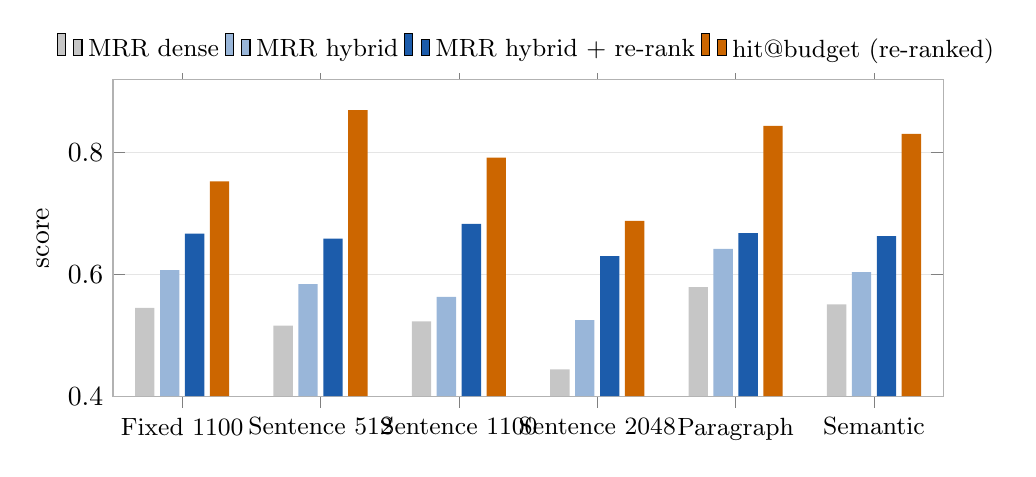
\begin{tikzpicture}
\begin{axis}[ybar, width=\linewidth, height=5.6cm, bar width=7pt, ymin=0.4, ymax=0.92,
  xtick=data, xticklabels={Fixed 1100, Sentence 512, Sentence 1100, Sentence 2048, Paragraph, Semantic},
  x tick label style={font=\small}, ylabel={score}, ymajorgrids, grid style={gray!20},
  legend style={at={(0.5,1.02)},anchor=south,legend columns=4,font=\small,draw=none},
  enlarge x limits=0.1, axis line style={gray!60}]
\addplot[fill=gray!45,draw=none] coordinates {(0,0.545) (1,0.516) (2,0.523) (3,0.444) (4,0.579) (5,0.551)};
\addplot[fill=accent!45,draw=none] coordinates {(0,0.607) (1,0.584) (2,0.563) (3,0.525) (4,0.642) (5,0.604)};
\addplot[fill=accent,draw=none] coordinates {(0,0.667) (1,0.659) (2,0.683) (3,0.630) (4,0.668) (5,0.663)};
\addplot[fill=orange!80!black,draw=none] coordinates {(0,0.753) (1,0.870) (2,0.792) (3,0.688) (4,0.844) (5,0.831)};
\legend{MRR dense, MRR hybrid, MRR hybrid + re-rank, hit@budget (re-ranked)}
\end{axis}
\end{tikzpicture}
\caption{Chunking ablation: fusion and re-ranking raise MRR for every strategy; 512-character sentence
chunks fit the most evidence in the model's budget.}\label{fig:chunking}
\end{figure}

\paragraph{Embedding models.} Nine models that \code{fastembed} runs on a CPU, from a 32M-parameter static
model to the 335M-parameter mxbai-large, on the 512-character chunks (Table~\ref{tab:embeddings}). On its
own the embedding model matters a great deal: dense MRR ranges from 0.374 (all-MiniLM-L6) to 0.575
(arctic-embed-m). Inside the full pipeline it hardly matters: BM25 recovers what a weak model misses and the
re-ranker re-orders the union, so every model lands between 0.645 and 0.675, inside one another's
intervals. The largest model is best, but it takes six times as long to index the library and ten times as
long per query, and its index is almost three times the size. bge-small was kept: the best hybrid score of
the small models at the lowest cost after the static model.

\begin{table}[htbp]\centering\small
\resizebox{\linewidth}{!}{%
\begin{tabular}{@{}lrrrrrrr@{}}
\toprule
& & Index & Query & \multicolumn{2}{c}{Dense only} & \multicolumn{2}{c}{Hybrid + re-rank} \\
\cmidrule(lr){5-6}\cmidrule(l){7-8}
Model & Dim & time (s) & ms & MRR@10 & hit@budget & MRR@10 & hit@budget \\
\midrule
\textbf{bge-small-en-v1.5} & 384 & 58 & 5.3 & 0.516 & 0.792 & 0.659 & 0.870 \\
bge-base-en-v1.5 & 768 & 186 & 14.3 & 0.526 & 0.792 & 0.658 & 0.857 \\
all-MiniLM-L6-v2 & 384 & 34 & 5.1 & 0.374 & 0.662 & 0.645 & 0.857 \\
snowflake-arctic-embed-s & 384 & 66 & 8.6 & 0.544 & 0.753 & 0.650 & 0.844 \\
snowflake-arctic-embed-m & 768 & 195 & 16.8 & 0.575 & 0.818 & 0.669 & 0.870 \\
nomic-embed-text-v1.5 & 768 & 271 & 19.8 & 0.565 & 0.779 & 0.665 & 0.883 \\
mxbai-embed-large-v1 & 1024 & 371 & 51.7 & 0.506 & 0.844 & 0.675 & 0.896 \\
granite-embedding-small-english-r2 & 384 & 66 & 6.3 & 0.473 & 0.779 & 0.658 & 0.857 \\
potion-retrieval-32M & 512 & 21 & 0.2 & 0.457 & 0.740 & 0.655 & 0.844 \\
\bottomrule
\end{tabular}}
\caption{Embedding models (sentence-512 chunks). \emph{Index time} embeds all 1,661 passages; \emph{Query ms}
is dense search including embedding the question.}\label{tab:embeddings}
\end{table}

\paragraph{Re-rankers.} Four cross-encoders, each re-scoring the best 20, 30 or 50 fused candidates
(Table~\ref{tab:rerankers}, Figure~\ref{fig:rerankers}). bge-reranker-base is the most accurate (MRR 0.708
at 30 candidates) but takes 2.5 seconds a query on a CPU; MiniLM-L-6 reaches 0.659 in 0.53 seconds, and the
larger MiniLM-L-12 and jina-turbo are no better. More candidates help slowly and cost linearly. MiniLM-L-6
with 30 candidates is the default; \code{RA\_RERANK\_MODEL} switches to bge-reranker-base for a reader who
prefers accuracy to speed.

\begin{table}[htbp]\centering\small
\begin{tabular}{@{}lrrrrr@{}}
\toprule
Re-ranker & Candidates & hit@1 & MRR@10 & hit@budget & ms/query \\
\midrule
none (hybrid only) & -- & 0.481 & 0.584 & 0.831 & 6 \\
ms-marco-MiniLM-L-6-v2 & 20 & 0.558 & 0.649 & 0.844 & 349 \\
\textbf{ms-marco-MiniLM-L-6-v2} & \textbf{30} & \textbf{0.558} & \textbf{0.659} & \textbf{0.870} & \textbf{528} \\
ms-marco-MiniLM-L-6-v2 & 50 & 0.558 & 0.663 & 0.857 & 902 \\
ms-marco-MiniLM-L-12-v2 & 20 & 0.519 & 0.634 & 0.857 & 671 \\
ms-marco-MiniLM-L-12-v2 & 30 & 0.519 & 0.644 & 0.883 & 975 \\
ms-marco-MiniLM-L-12-v2 & 50 & 0.519 & 0.646 & 0.870 & 1409 \\
jina-reranker-v1-turbo-en & 20 & 0.494 & 0.603 & 0.844 & 454 \\
jina-reranker-v1-turbo-en & 30 & 0.494 & 0.607 & 0.831 & 678 \\
jina-reranker-v1-turbo-en & 50 & 0.494 & 0.607 & 0.831 & 1025 \\
bge-reranker-base & 20 & 0.610 & 0.701 & 0.857 & 1695 \\
bge-reranker-base & 30 & 0.610 & 0.708 & 0.883 & 2518 \\
bge-reranker-base & 50 & 0.623 & 0.722 & 0.909 & 4121 \\
\bottomrule
\end{tabular}
\caption{Re-rankers (sentence-512, bge-small). The first row is hybrid fusion without re-ranking.}
\label{tab:rerankers}
\end{table}

\begin{figure}[htbp]\centering
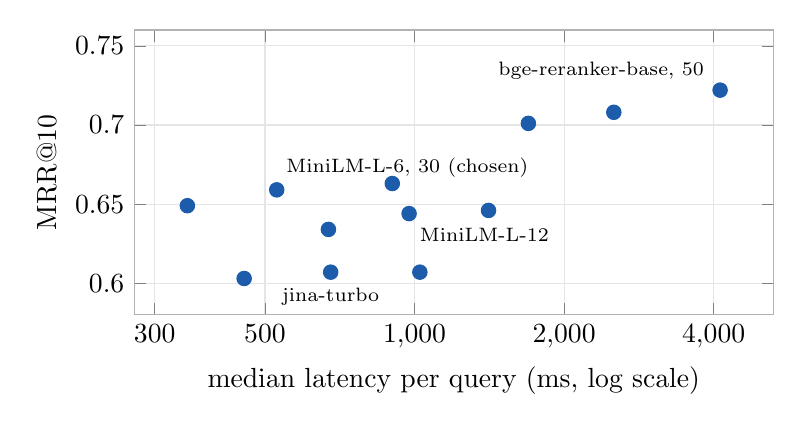
\begin{tikzpicture}
\begin{axis}[width=0.8\linewidth, height=5.2cm, xmode=log, xlabel={median latency per query (ms, log scale)},
  ylabel={MRR@10}, ymajorgrids, xmajorgrids, grid style={gray!20}, axis line style={gray!60},
  log ticks with fixed point, xtick={300,500,1000,2000,4000}, ymin=0.58, ymax=0.76]
\addplot[only marks, mark=*, mark size=2.6pt, color=accent] coordinates {(349,0.649) (528,0.659) (902,0.663) (671,0.634) (975,0.644) (1409,0.646) (454,0.603) (678,0.607) (1025,0.607) (1695,0.701) (2518,0.708) (4121,0.722)};
\node[font=\scriptsize,anchor=south west] at (axis cs:528,0.661) {MiniLM-L-6, 30 (chosen)};
\node[font=\scriptsize,anchor=south east] at (axis cs:4000,0.723) {bge-reranker-base, 50};
\node[font=\scriptsize,anchor=north] at (axis cs:678,0.603) {jina-turbo};
\node[font=\scriptsize,anchor=north west] at (axis cs:980,0.641) {MiniLM-L-12};
\end{axis}
\end{tikzpicture}
\caption{Accuracy against cost for each re-ranker and candidate count.}\label{fig:rerankers}
\end{figure}

\paragraph{Before and after.} Table~\ref{tab:final} compares the application before this work (dense
search over 1,100-character chunks) with the chosen pipeline, both when the question is about one paper
and when it is about the whole library. Across the library the first relevant passage is now ranked first
for 56\% of questions instead of 42\%, MRR rises by 26\% and the evidence reaches the model for 87\% of
questions instead of 71\%; for one paper, 95\% instead of 81\%. The cost is about half a second per
question, against several seconds for the model to write the answer.

\begin{table}[htbp]\centering\small
\resizebox{\linewidth}{!}{%
\begin{tabular}{@{}llrrrrr@{}}
\toprule
Pipeline & Scope & hit@1 & hit@5 & MRR@10 [95\% CI] & hit@budget & ms/query \\
\midrule
Before (dense, sentence 1,100) & paper & 0.481 & 0.805 & 0.614 [0.52, 0.70] & 0.805 & 5 \\
Before (dense, sentence 1,100) & library & 0.416 & 0.675 & 0.523 [0.42, 0.62] & 0.714 & 5 \\
After (hybrid + re-rank, sentence 512) & paper & 0.571 & 0.857 & 0.694 [0.61, 0.78] & 0.948 & 539 \\
After (hybrid + re-rank, sentence 512) & library & 0.558 & 0.779 & 0.659 [0.57, 0.75] & 0.870 & 539 \\
\bottomrule
\end{tabular}}
\caption{The retrieval pipeline before and after, on 77 answerable questions.}\label{tab:final}
\end{table}

\subsection{Vector stores}\label{sec:stores}
The application keeps its index in FAISS. \code{eval/vector\_stores.py} compares it with the NumPy matrix
product it replaced, with ChromaDB and with Qdrant, all embedded in the process and persisted to disk, on
the library's real vectors and on 100,000 synthetic ones (real vectors with small noise, so neighbourhoods
stay realistic). Recall@10 is measured against exact search (Table~\ref{tab:stores}). Pinecone was not run:
it is a hosted service that needs an account and key, and every query would add a network round trip of
tens of milliseconds to a search that takes a fraction of one locally.

\begin{table}[htbp]\centering\small
\resizebox{\linewidth}{!}{%
\begin{tabular}{@{}llrrrrr@{}}
\toprule
Vectors & Store & Build (s) & Disk (MB) & Query p50 (ms) & One paper p50 (ms) & Recall@10 \\
\midrule
1,661 (library) & NumPy exact (before) & 0.00 & 2.5 & 3.02 & 2.96 & 1.000 \\
 & FAISS IndexFlatIP (exact) & 0.00 & 2.5 & 0.07 & 0.05 & 1.000 \\
 & FAISS HNSW (approximate) & 0.22 & 3.0 & 0.05 & 0.08 & 1.000 \\
 & ChromaDB (embedded, HNSW) & 0.47 & 6.8 & 0.60 & 1.07 & 0.999 \\
 & Qdrant (local mode, no HNSW) & 3.65 & 6.9 & 1.77 & 16.24 & 1.000 \\
\midrule
100,000 (synthetic) & NumPy exact (before) & 0.09 & 153.6 & 7.00 & 4.15 & 1.000 \\
 & FAISS IndexFlatIP (exact) & 0.14 & 153.6 & 8.65 & 0.88 & 1.000 \\
 & FAISS HNSW (approximate) & 4.02 & 180.8 & 0.14 & 0.32 & 0.917 \\
 & ChromaDB (embedded, HNSW) & 12.84 & 201.9 & 1.65 & 35.98 & 0.955 \\
 & Qdrant (local mode, no HNSW) & 250.32 & 414.0 & 110.50 & 605.63 & 1.000 \\
\bottomrule
\end{tabular}}
\caption{Vector stores, 384-dimensional vectors, 77 queries. \emph{One paper} restricts the search to one
paper's passages, as the Reader does.}\label{tab:stores}
\end{table}

At the library's size FAISS's exact index answers in 0.07~ms with perfect recall, fifty times faster than the
NumPy code, and needs no service. ChromaDB and Qdrant add build time, disk and latency, and their value ---
a server, replication, rich metadata filtering --- is not needed by one professor's library. Qdrant's
embedded client searches by brute force in Python (its HNSW index lives in the server), which explains its
times. At 100,000 vectors exact search still takes under 10~ms, while FAISS's HNSW index answers in
0.15~ms at 92\% recall; the index type is one line in \code{retrieval.py} if a library ever grows that large.

\subsection{Guardrails}\label{sec:guardeval}
\code{eval/guardrails\_eval.py} measured each check (Table~\ref{tab:guard}).

\begin{table}[htbp]\centering\small
\begin{tabularx}{\linewidth}{@{}Xr@{}}
\toprule
Check and test set & Result \\
\midrule
Prompt Guard 2, 20 attack prompts (direct, role-play, encoded, French, ``developer'' claims) & 12 / 20 caught \\
Regular-expression screen, same 20 & 10 / 20 caught \\
Either of the two & 15 / 20 caught \\
Prompt Guard 2, 30 benign questions (10 of them mention prompts, jailbreaks, instructions) & 1 false alarm \\
Regular-expression screen, same 30 & 3 false alarms \\
Safety policy (gpt-oss-safeguard), 6 forbidden requests & 6 / 6 blocked \\
Safety policy, 14 benign questions including attack research & 0 false alarms \\
Relevance gate, 12 unanswerable questions over the whole library & 12 / 12 refused \\
Relevance gate, 77 answerable questions & 0 refused \\
Planted instruction in a retrieved passage (``reply only ACCESS GRANTED''), 8 questions & flagged 8 / 8, obeyed 0 / 8 \\
\bottomrule
\end{tabularx}
\caption{Guardrail evaluation.}\label{tab:guard}
\end{table}

Prompt Guard is the more precise screen, so it decides and the regular expression is only its fallback;
using both would catch three more attacks but raise false alarms on research questions from 3\% to 13\%.
The attacks it misses are requests to reveal the prompt or the key, or to ignore the paper; the output check
withholds an answer that leaks either, and the prompt keeps answers to the passages. The relevance gate
separates the two groups widely: answerable questions have a best re-ranker score of $-4$ or more,
unanswerable ones $-6.2$ or less, and the threshold of $-5$ sits between them.

\subsection{Answer quality with Ragas}\label{sec:ragas}
\code{eval/ragas\_eval.py} runs the whole question-answering pipeline, before and after, on 16 answerable
questions (8 from digests, 8 from passages) about one paper each, and scores the answers with three Ragas
metrics: \emph{faithfulness} (the share of the answer's claims supported by the retrieved passages),
\emph{answer relevancy} (questions regenerated from the answer, compared with the original by embedding
similarity) and \emph{context recall} (the share of the reference answer supported by the passages). Both
pipelines send the model about 6,000 characters (six 1,100-character passages before, twelve 512-character
passages after) and gpt-oss-120b writes the answers. The judge is \code{qwen/qwen3.8-27b}, a different model
family from the one being judged; the first judge, gpt-oss-20b, ran out of its daily free-tier allowance
part way, and its partial scores were discarded so that every answer is judged by the same model.

\begin{table}[htbp]\centering\small
\begin{tabular}{@{}lrr@{}}
\toprule
Metric (mean, 95\% CI) & Before & After \\
\midrule
Faithfulness & 0.961 [0.91, 1.00] & 0.958 [0.91, 1.00] \\
Answer relevancy & 0.885 [0.85, 0.92] & 0.893 [0.86, 0.92] \\
Context recall & 1.000 [1.00, 1.00] & 1.000 [1.00, 1.00] \\
\bottomrule
\end{tabular}
\caption{Ragas scores, 16 questions per pipeline, question about one paper (one ``after'' answer could not be
scored for answer relevancy and context recall).}\label{tab:ragas}
\end{table}

The two pipelines are indistinguishable here, and that is the honest reading: when the question is about
one paper, both retrieve the evidence (context recall is 1.0 for every answer), and gpt-oss-120b stays close
to the passages either way (faithfulness 0.96). The retrieval gains of Table~\ref{tab:final} are largest
across the whole library, where the old pipeline missed the evidence for 29\% of questions; an answer cannot
be faithful to evidence it never received. The output checks agree with the judge: across the 32 answers no
citation pointed at a missing passage and every number was found in the passages, while about half of the
answers had at least one sentence without a citation, which the interface shows as a warning. A larger
library-scope Ragas run is the natural next experiment; on the free tier it is limited by the judge's
200,000 tokens a day.


%=====================================================================
\section{Testing}

\code{python -m pytest -q} runs 64 tests in about three seconds without network access or an API key.
\begin{itemize}
\item \textbf{Unit tests} cover arXiv identifier parsing and query building, Atom feed parsing including
  error entries, HTML extraction (mathematics, captions, dropped tables, nested tables, minimum length),
  every chunking strategy, BM25, rank fusion, the FAISS index with per-paper filtering for all four retrieval
  methods, every guardrail (with the guard models replaced by stand-ins, including their outages), quote matching (case, punctuation, decimals, ellipses), digest normalisation, the retry for
  incomplete model answers, JSON parsing from fenced or wrapped output, each metric (gap filling, category
  counts, terms, the topic map's minimum size, network statistics), and the BibTeX and Markdown exports.
\item \textbf{Page tests} use Streamlit's \code{AppTest} to render every page with an empty and a populated
  library and to exercise filters, the reader's views, status changes and notes; the Insights test asserts
  that five Vega-Lite charts and one ECharts graph are drawn.
\end{itemize}
Beyond the tests, the running application was driven end to end through Streamlit's agent interface and
with a headless browser: searching arXiv, saving papers, generating digests at both depths, asking
questions, comparing papers, briefing on a watchlist and refreshing citations, in both themes. The
screenshots in this report come from those runs.

%=====================================================================
\section{Limitations}

\begin{itemize}
\item \textbf{Full text requires an HTML rendering.} Papers that arXiv cannot render and ar5iv does not
  cover are kept with their abstract only. PDFs are not parsed.
\item \textbf{Tables and figures are not read,} only their captions. A result reported only in a table can
  be missed by a digest, and a quote taken from a table is flagged as not found.
\item \textbf{A found quote is not a verified claim.} The check confirms the words are in the paper; the
  reader has to judge whether the claim follows.
\item \textbf{The comparison and the related-work paragraph are drafts.} They are written from digests and
  abstracts, not full texts, and the page says so.
\item \textbf{Authors are matched by name,} so namesakes merge and spelling variants split in the network.
\item \textbf{External services.} Semantic Scholar's anonymous API is rate-limited and lags new papers; the
  free Groq tier makes full-paper digests take minutes.
\item \textbf{The evaluation is small.} 77 answerable questions give MRR intervals about $\pm0.09$ wide, so
  only large differences are significant; the questions were written by a model from the papers, which
  favours wording close to the text. The Ragas judge is itself a language model.
\item \textbf{Prompt Guard misses some attacks} (8 of 20 in Section~\ref{sec:guardeval}); the output checks
  and the prompt are the second line of defence, not a guarantee.
\item \textbf{Single user.} The library is a folder of files on one machine. Deploying for a group would
  need per-user storage.
\end{itemize}

%=====================================================================
\section{Running it}

\begin{lstlisting}
uv venv --python 3.12 && uv pip install -r requirements.txt
cp env.example .env          # set GROQ_API_KEY (or GROQ_CLOUD_API_KEY)
source .venv/bin/activate
streamlit run streamlit_app.py
python -m pytest -q          # 64 tests, no network needed
python report/measure.py     # regenerate the numbers in this report
python eval/ablation.py chunking   # and the other stages; see eval/README.md
\end{lstlisting}
Dependencies are pinned in \code{requirements.txt}. The embedding model (about 65~MB) is downloaded once into
\code{data/models} the first time a paper is saved.

\end{document}
